\section{Random walks}

A random walker is a point object which after a certain amount of time jumps a fixed step length either right or left with equal probability for jumping either way. 
In $d$ spatial dimensions the axis on which the jump happens is chosen at random before the direction of the jump is decided. \\
Say a distribution of random walkers, $C$ is chosen so that all the walkers are placed within an imagined volume, $V$ of arbitrary shape. 
$V$ is contained by a surface $S$ and the relation is shown in Figure \ref{theory:divergence_theorem}. 

\begin{figure}[H]
\centering
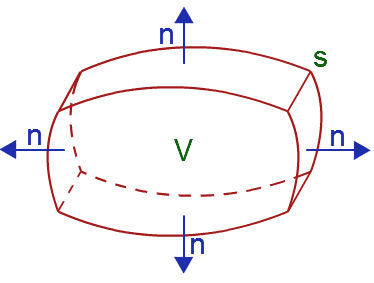
\includegraphics[scale=0.6]{Figures/divergence_theorem.png}
 \caption[]{}
 \label{theory:divergence_theorem}
\end{figure}

\noindent As the random walkers start to move some of them will leave the volume $V$ which results in a change in $C$. 
The net movement of random walkers at a point is called the flux of walkers and is denoted by the flux vector $\mathbf J$. 
To find the number of walkers that leave $V$ we integrate the normal component of $\mathbf J$ over $S$. 
Assuming that no walkers disappear or are created the flux of walkers leaving $V$ must be balanced by the decrease in $C$, expressed in equation \eqref{theory:diffusion_integral_form}. 

\begin{equation}\label{theory:diffusion_integral_form}
 \int_V \frac{\d C}{\d t}\,dV = \int_S\vec{J}\cdot \vec{n}\,dS
\end{equation}

\noindent Through Greens theorem equation \eqref{theory:diffusion_integral_form} can be reformulated

\begin{equation}\label{theory:integral_form}
 \int_V \frac{\d C}{\d t}\,dV = \int_V\nabla\cdot\vec{J}\,dV
\end{equation}

\noindent The flux $\vec{J}$ can be expressed by Fick's first law as the diffusive flux 
\begin{equation}
 \vec J = D\nabla C
\end{equation}

\noindent where $D$ is the diffusion constant. Since $V$ was chosen as an arbitrary volume equation \eqref{theory:integral_form} is independent of the integration and the integrals can be dropped. 
The diffusive flux $\mathbf{J}$ is also inserted to yield the diffusion equation

\begin{equation}\label{theory:diffusion_equation}
 \frac{\d C}{\d t} = D\nabla^2 C
\end{equation}

\noindent Throughout this thesis $C$ will denote a spatial distribution of random walkers. 
$C$ is best illustrated in Figure \ref{theory:illustration_C}.

\begin{figure}[H]
 \centering
 \begin{subfigure}{0.48\textwidth}
  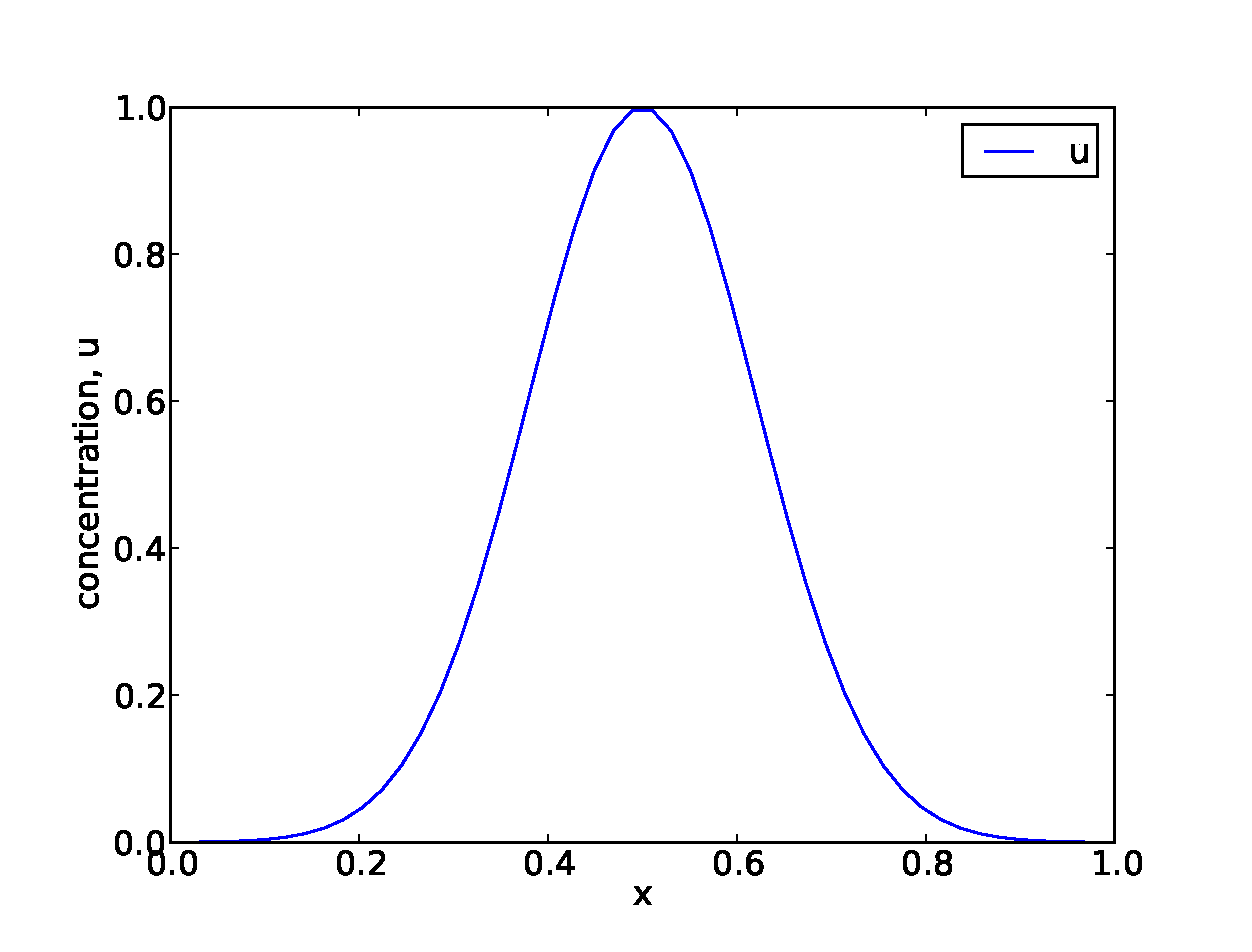
\includegraphics[width=\textwidth]{Figures/illustration_C_pt1.eps}
  \caption{}
 \end{subfigure}
 \begin{subfigure}{0.48\textwidth}
  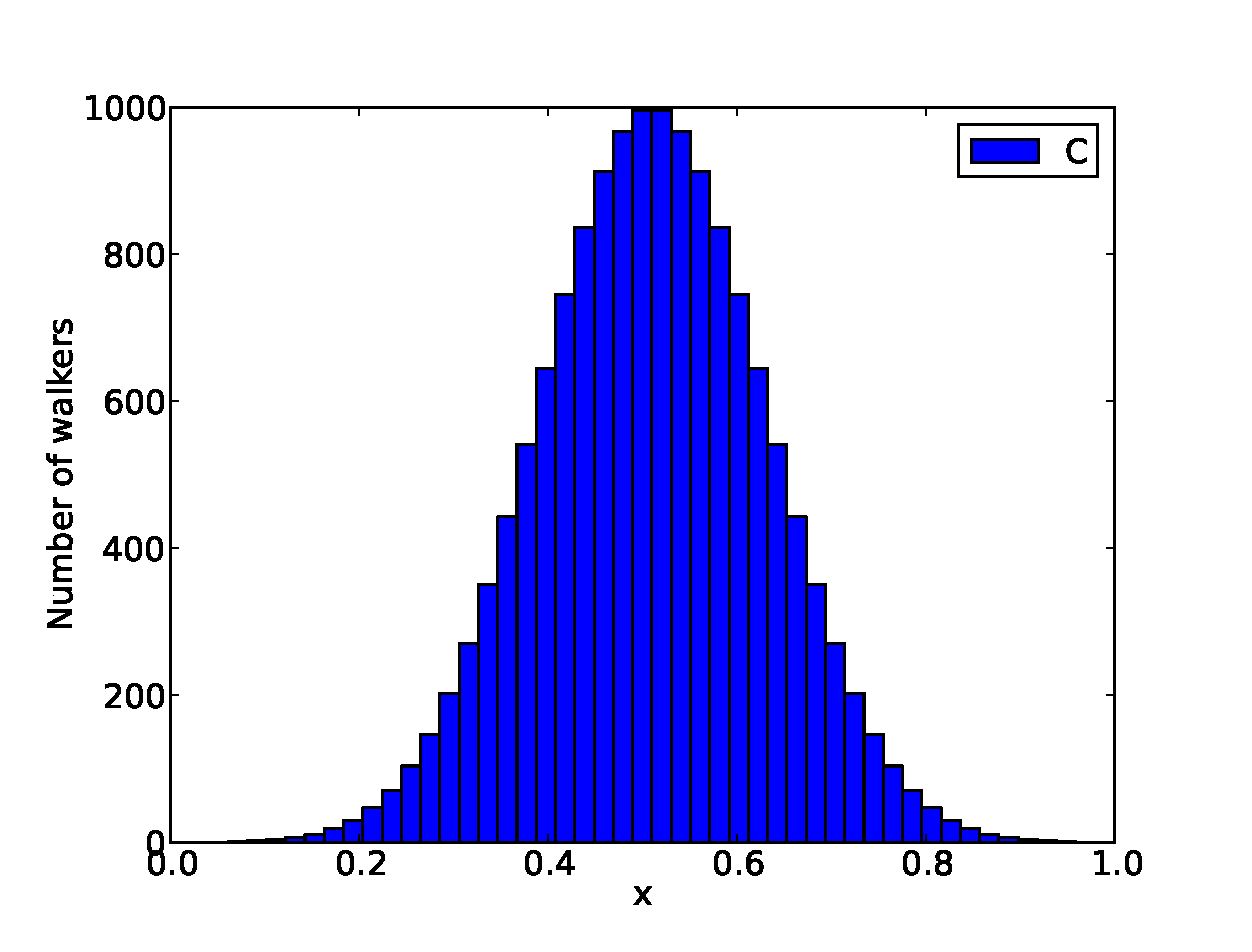
\includegraphics[width=\textwidth]{Figures/illustration_C_pt2.eps}
  \caption{}
 \end{subfigure}
 \caption[Illustration of $C(x)$]{Illustration of the difference between $u(x,t)$ in (a) which is the solution to the diffusion equation and $C(x,t)$ in (b) which is the number of random walkers within an area of $\pm\frac{\Delta x}{2}$ around each mesh point.}
 \label{theory:illustration_C}
\end{figure}


\subsection{Random number generator}

To produce a random walk one must have random numbers. 
The random numbers in this thesis are produced by a five seeded xor-shift algorithm copied from George Marsaglia \cite{marsaglia2003xorshift}. 
This generator is chosen because of its very large period ($\sim10^{48}$) compared to the computational cost.

\section{Backward Euler schemes in 2 or more spatial dimensions}

The reader is assumed to know the basics of solving partial differential equations (PDEs\nomenclature{PDE}{Partial Differential Equation}) by finite difference methods, but for the sake of clarity the two schemes used in this thesis are written out. 
\begin{equation}\label{theory_theta_rule}
 \frac{u^{n+1}-u^n}{\Delta t} = \theta D\frac{\d^2 u^{n+1}}{\d x^2} + (1-\theta)D\frac{\d^2 u^{n}}{\d x^2}
\end{equation}
\noindent Having $\theta = 0$ gives the Forward Euler (FE\nomenclature{FE}{Forward Euler}) scheme, and $\theta = 1$ gives the  Backward Euler (BE\nomenclature{BE}{Backward Euler}) scheme. \\
This section will concern a simple, but elegant way of efficiently solving the diffusion equation by the implicit BE scheme in more than one spatial dimension. 
% This section will concern the special case of how to solve the diffusion equation by the implicit BE scheme, especially in more than one spatial dimension.
First, let us look at the BE discretization of the diffusion equation in 1D. 

\begin{align}\label{theory:BE_scheme_1D}
 u^{n+1}_i = \frac{\Delta t}{2\Delta x^2}\left((D_{i+1}+D_{i})(u^{n+1}_{i+1}-u^{n+1}_{i})-(D_{i}+D_{i-1})(u^{n+1}_{i}-u^{n+1}_{i-1})\right) + u^n_i
\end{align}
$u$ is here the unknown function which solves the diffusion equation. 
Note that 
$$u^n_i = u(t_0+n\cdot\Delta t,x_0+i\cdot\Delta x)$$
and not $u$ to the $n$'th power. \\
Neumann boundary conditions will be used, these are described in \eqref{theory:Neumann_boundaries}.

\begin{equation}\label{theory:Neumann_boundaries}
 \frac{\d u}{\d n} = 0|_{\text{on boundary}}
\end{equation}

\noindent Solving the BE scheme by hand for a very small mesh consisting of $4$ mesh points will reveal the structure of the BE scheme.
\begin{align*}
 &u^{n+1}_0 =  \frac{\Delta t}{2\Delta x^2}\left(2(D_{0}+D_{1})(u^{n+1}_{1}-u^{n+1}_{0})\right) + u^n_0\\
 &u^{n+1}_1 = \frac{\Delta t}{2\Delta x^2}\left((D_{2}+D_{1})(u^{n+1}_{2}-u^{n+1}_{1})-(D_{1}+D_{0})(u^{n+1}_{1}-u^{n+1}_{0})\right) + u^n_1\\
 &u^{n+1}_2 = \frac{\Delta t}{2\Delta x^2}\left((D_{3}+D_{2})(u^{n+1}_{3}-u^{n+1}_{2})-(D_{2}+D_{1})(u^{n+1}_{2}-u^{n+1}_{1})\right) + u^n_2 \\
 &u^{n+1}_3 =  \frac{\Delta t}{2\Delta x^2}\left(2(D_{2}+D_{3})(u^{n+1}_{3}-u^{n+1}_{2})\right) + u^n_3
\end{align*}

\noindent Rearranging this and setting $a = \frac{\Delta t}{2\Delta x^2}$ results in a normal system of linear equations
\begin{align*}
 &u^{n+1}_0\left(1+2a(D_0+D_1)\right)- 2au^{n+1}_{1}(D_1+D_0) =  u^n_0\\
 &u^{n+1}_1\left(1+a(D_2+2D_1+D_0)\right)-au^{n+1}_{2}(D_2+D_1)-au^{n+1}_{0}(D_1+D_0) = u^n_1\\
 &u^{n+1}_2\left(1+a(D_3+2D_2+D_1)\right)-au^{n+1}_{3}(D_3+D_2)-au^{n+1}_{1}(D_2+D_1) = u^n_2\\
 &u^{n+1}_3\left(1+2a(D_3+D_2)\right)- 2au^{n+1}_{2}(D_3+D_2) =  u^n_3
\end{align*}
which is arranged as 

\begin{align}\label{BE}
 \left(\begin{array}{c c c c}
        b_0 & c_0 &0 &0 \\
        a_1 & b_1 & c_1 &0 \\
        0& a_2 & b_2& c_2\\
        0& 0& a_3 & b_3\\
       \end{array}\right)\mathbf{u}^{n+1} = \mathbf{u}^{n}
\end{align}
\noindent The coefficient matrix in \eqref{BE} will be labeled $\mathbf M$ throughout the thesis.
\begin{equation}\label{theory:BE:linear_system}
  \mathbf{M}\mathbf{u}^n = \mathbf{u}^{n-1}
\end{equation}

\noindent If a linear system like the one in \eqref{theory:BE:linear_system} has a solution it can always be found by Gaussian elimination \textcolor{red}{check this}. 
However, for a sparse linear system a lot of the calculations in a Gaussian elimination will be done with zeros. 
A dramatically more efficient way to solve the linear system in \eqref{theory:BE:linear_system} is by exploiting the fact that it is tridiagonal. 
In order to be more consistent with the algorithm, \eqref{theory:BE:linear_system} will be rewritten as
\begin{equation}
  \mathbf{M}\mathbf{u} = \mathbf{up}
\end{equation}
where $\mathbf{up}$ denotes the solution $\mathbf{u}$ at the previous time step. 
Tridiagonal systems can be solved extremely efficiently by the ``tridiag`` algorithm listed below.

\lstinputlisting{Figures/tridiag.cpp}

In two spatial dimensions the BE discretization gives the scheme shown in equation \eqref{general_scheme_BE2D}

\begin{equation}\label{general_scheme_BE2D}
 u^{n}_{i,j} = \underbrace{\frac{-D\Delta t}{\Delta x^2}}_{\alpha}\left(u^{n+1}_{i+1,j}+u^{n+1}_{i-1,j}\right) +
 \underbrace{\left(1+\frac{2D\Delta t}{\Delta x^2} +\frac{2D\Delta t}{\Delta y^2}\right)}_{\gamma}u^{n+1}_{i,j} 
 \underbrace{-\frac{2D\Delta t}{\Delta y^2}}_{\beta}\left(u^{n+1}_{i,j+1}+u^{n+1}_{i,j-1}\right)
\end{equation}

\noindent If \eqref{general_scheme_BE2D} is solved by hand on a $3\times3$ mesh by the same steps as in 1D it gives the following linear system
% \noindent Equation \eqref{general_scheme_BE2D} assembles to the linear system in equation \eqref{linear_system_BE2D} when solved on a $3\times3$ mesh.
\begin{align}\label{linear_system_BE2D}
  \left(\begin{array}{c c c : c c c : c c c}
        \gamma & -2\beta &0 &-2\alpha &0 &0 &0 &0 &0\\
        -\beta & \gamma & -\beta &0 &-2\alpha &0 &0 &0 &0\\
        0&-2\beta & \gamma & 0 & 0 & -2\alpha &0&0&0\\ \hdashline
        -\alpha& 0&0 & \gamma & -2\beta & 0 & -\alpha &0&0\\
        0& -\alpha&0&-\beta & \gamma & -\beta & 0 & -\alpha &0\\
        0& 0& -\alpha&0&-2\beta & \gamma & 0 & 0 &-\alpha\\ \hdashline
        0& 0 &0 &-2\alpha &0&0 & \gamma & -2\beta&0\\
        0& 0 &0 &0 &-2\alpha&0&-\beta & \gamma &-\beta\\
         0&0 &0 &0&0 &-2\alpha&0&-2\beta & \gamma
       \end{array}\right)\mathbf{u}^{n+1} = \mathbf{u}^{n}
\end{align}

\noindent The dashed lines confine a total of nine $3\times 3$ matrices which can be used to reformulate the $2n +1 = 7$ band diagonal system as a block tridiagonal system as shown below.
\begin{align}\label{block_tridiagonal_dashed}
 \left(\begin{array}{c : c : c }
        B_0 & C_0 &0  \\ \hdashline
        A_1 & B_1 & C_1 \\ \hdashline
        0& A_2 & B_2
       \end{array}\right)\mathbf{u}^{n+1} = \mathbf{u}^{n}
\end{align}

\noindent All entries in eq. \eqref{block_tridiagonal_dashed} are $3\times3$ matrices. 
In the general case where the diffusion equation is discretized and solved on a mesh of size $n\times n$ the resulting block tridiagonal system will consist of $n^2$ matrix entries which all are $n\times n$ matrices.
% In two spatial dimensions the BE discretization will result in a a $2n$ band diagonal matrix of size $n^2\times n^2$ with 5 nonzero bands. 
% This band diagonal matrix can be rewritten as a block tridiagonal matrix with $n\times n$ matrices as entries. 
% A simplified block tridiagonal linear system is shown in eq. \eqref{theory:block_tridiagonal_matrix}
% 
% 
% \begin{align}\label{theory:block_tridiagonal_matrix}
%    \left(\begin{array}{c c c c c c c c c}
%         B_0 & C_0 &0 &0 &0 &0 &0 &0 &0\\
%         A_1 & B_1 & C_1 &0 &0 &0 &0 &0 &0\\
%         0&\ddots & \ddots & 0 & 0 & \ddots &0&0&0\\
%         0 & 0&A_i & B_i & C_i& 0 &  &0&0\\
%         0& \ddots&0&\ddots & \ddots & \ddots & 0 & \ddots &0\\
%          0&0 &0 &0&0 &0&0&A_{n-1} & B_{n-1}
%        \end{array}\right) \left(\begin{array}{c}
%              \mathbf{u}^{n+1}_{0}\\
%              \mathbf{u}^{n+1}_{1}\\
%              \vdots\\
%              \mathbf{u}^{n+1}_{i}\\
%              \vdots\\
%              \mathbf{u}^{n+1}_{n}
%              \end{array}\right) = \mathbf{up}
% \end{align}

One should note that the $n\times n$ matrix $\mathbf u$ which solves the 2D diffusion equation has be rewritten as a vector $\mathbf{u}$ of size $n^2$. \\ 

In order to solve this block tridiagonal linear system the ''tridiag`` solver from before must be generalized to support matrices as entries in $\mathbf M$. 
Luckily this generalization is trivial and all that is needed is to replace divisions by matrix inverses. 
An updated \emph{pseudo coded} scheme is listed in \eqref{block_tridiag_alg}

There is a forward substitution
\begin{align}\label{block_tridiag_alg}
 H_0 &= -B_0^{-1}C_0\nonumber \\
 \mathbf{g}_0 &= B_0^{-1}\mathbf{up}_0 \nonumber\\
 H_i &= -\left(B_i+A_iH_{i-1}\right)^{-1}C_i \nonumber \\
 \mathbf{g}_i &= \left(B_i+A_iH_{i-1}\right)^{-1}\left(\mathbf{up}_i-A_i\mathbf{g}_{i-1}\right)
 \end{align}
 Followed by a backward substitution
 \begin{align*}
  \mathbf{x}_{n-1} &= \mathbf{g}_{n-1}\nonumber\\
  \mathbf{x}_i &= \mathbf{g}_i + H_i\mathbf{x}_{i+1} \nonumber
 \end{align*}
 
 It is possible to solve the BE scheme in 3D by the block tridiagonal solver as well. 
 The linear system will be $2n^2 +1$ band diagonal and must first be reduced to a block matrix which is $2n+1$ band diagonal like the one in eq. \eqref{linear_system_BE2D} before it is further reduced to a block tridiagonal form. 
 Matrix entries will be $n^2\times n^2$ matrices.
 
 \subsubsection{Efficiency of the block tridiagonal algorithm}
 
 In general the Forward Euler (FE\nomenclature{FE}{Forward Euler}) scheme will solve a discrete PDE in $d$ spatial dimensions with $n$ mesh points in each dimension using
 \begin{equation*}
  \mathcal O(n^d)
 \end{equation*}
floating point operations (FLOPs\nomenclature{FLOPs}{Floating Point Operations (per second)}). 
This is the maximum efficiency possible for a PDE in $d$ dimensions (without using some form of symmetry argument) and will be the benchmark for the BE scheme as well.\\

Implicit schemes like BE result in linear systems which can be solved by multiplying both sides of the equation with the inverse of the matrix in question. 
\begin{equation*}
 \mathbf M^{-1}\mathbf M\mathbf u = \mathbf{M}^{-1}\mathbf{up}
\end{equation*}
Inverting a dense matrix demands $\mathcal O(n^3)$ FLOPs for an $n\times n$ matrix. 
By rewriting the previously mentioned $n^2\times n^2$ band diagonal matrix as a block tridiagonal matrix and using the modified block tridiagonal solver we have reduced the demanded number of FLOPs from $\mathcal{O}(n^6)$ to $n\cdot\mathcal{O}(n^3) = \mathcal{O}(n^4)$. 
Though an improvement of 2 orders is very good, compared to the FE scheme this is still one order larger.
there is still room for improvement, however. 
As long as the mass matrix is unchanged, which it will be as long as the time step and diffusion constant are constant, the $n$ matrix inversions need only be done once. 
In other words, the $H_i$ terms from eq. \eqref{block_tridiag_alg} can be stored. 
The remaining calculations include three matrix vector multiplications, all of which demand $n^2$ FLOPs, thus further reducing the computational cost to $\mathcal{O}(n^2)$ FLOPs which is the same as the FE scheme.

\section{Combining micro and macro scale models}

\subsection{The algorithm}
After setting an initial condition and diffusion constant the diffusion problem is solved on both the microscopic and macroscopic meshes and combined into a common solution by the following steps.
\begin{itemize}
 \item The result from previous PDE time step, $\mathbf{up}$, is converted to a distribution of random walkers and sent to the RW solver
 \item The RW solver does a predefined number of micro scale time steps which correspond to one PDE time step
 \item The result from the RW solver is converted back to a concentration and this replaces the PDE solution
 \item $\mathbf{up}$ is then used as input to calculate the next time step
\end{itemize}

\subsection{The conversion between length scales}
As the previous section states the result from the last PDE time step is converted to a distribution of random walkers. 
This is done by specifying a conversion rate denoted $Hc$ (as was done by Plapp and Karma \cite{plapp2000multiscale}) which is defined in equation \eqref{theory:Hc_definition}

\begin{equation}\label{theory:Hc_definition}
 C_{ij} = Hc\cdot u_{ij}
\end{equation}

\noindent As before $u_{ij}$ is the solution to the 2D diffusion equation evaluated at $x_0 +i\Delta x$ and $y_0 +j\Delta y$, and $C_{ij}$ is the number of random walkers located in the rectangle defined by $x_i\pm\frac{\Delta x}{2}$ and $y_j\pm\frac{\Delta y}{2}$. 
Walkers are given a random position within this rectangle at the beginning of each PDE time step. 

Equation \eqref{theory:Hc_definition} effectively states that one ''unit`` of the solution $u$ will directly correspond to $Hc$ random walkers.

\subsection{Coupling the models through step length}

To ensure that the $\tau$ time steps performed by the RW solver sums up to one time step for the PDE solver a limitation must be imposed on the RW solver. 
This limitation can only be imposed on the step length of the random walkers, so the task at hand is to relate the step length to the PDE time step and $\tau$. \\
Through an Einstein relation the variance in position is coupled to the diffusion constant.
\begin{equation}\label{theory:einstein_relation}
 \langle\tilde{\Delta x}^2\rangle = 2Dd\tilde{\Delta t}
\end{equation}
Where $\tilde{\Delta t}$ is the time step for the random walkers which is exactly $\tilde{\Delta t} = \frac{\Delta t}{\tau}$. 
Similarly $\tilde{\Delta x}$ is the spatial resolution on the micro scale which is also the step length, $l$, for the random walkers. 
Rewriting equation \eqref{theory:einstein_relation} gives the final expression for the step length

\begin{equation}\label{theory:step_length}
 l = \sqrt{2dD\frac{\Delta t}{\tau}}
\end{equation}

\subsection{Boundary conditions for the random walk}


\section{Potential problems or pitfalls}\label{problems_and_pitfalls}
 
This section will identify and discuss a few obvious difficulties which might arise in this project. As far as possible solutions or workarounds will be presented, but some problems might not be solvable.

% \subsubsection{Different timescales}
% The time scales are coupled through the step length of the random walkers which is shown in equation \eqref{steplength}. 
% \begin{equation}\label{steplength}
%  l = \sqrt{2Dd\frac{\Delta t}{\tau}}
% \end{equation}
% 
% Here $\tau$ is the number of time steps taken on the microscopic scale for each time step on the PDE scale, $d$ is the number of spatial dimensions, and $\Delta t$ is the time step on the PDE scale. 


 
\subsubsection{Negative concentration of walkers}
Physically a negative concentration does not make sense, but if an initial condition which takes negative values is imposed on the system the software will try to allocate a negative number of walkers. 
Trying to handle this is more of an oddity than anything else, but a workaround has been found. 
If the absolute value of the negative concentration is taken as input to the RW solver and the sign at each mesh point is stored while the RW solver advances the system, the resulting solution can be multiplied by the stored sign to give back a negative concentration. 
The workaround will at least keep the simulation from crashing, but has a fundamental problem which is illustrated in Figure \ref{theory:signmap_illustration}.
  
\begin{figure}[H]
\centering
\begin{subfigure}[t!]{0.48\textwidth}
 \includegraphics[width=\textwidth]{Figures/signmap_illustration_pt1.eps}
 \caption{}
\end{subfigure}
\begin{subfigure}[t!]{0.48\textwidth}
 \includegraphics[width=\textwidth]{Figures/signmap_illustration_pt2.eps}
 \caption{}
\end{subfigure}
\caption[Workaround for negative concentrations, illustration]{An illustration of the proposed workaround for negative concentrations and an illustration of how well it works (b). The fundamental problem is that a diffusion process will even out discontinuities such as the one in (a). The result of this evening out is shown in (b) as an increase in concentration in the middle mesh point which should remain equal to zero.}
\label{theory:signmap_illustration}
 \end{figure}

\subsubsection{Smooth solutions}


\subsubsection{Number of time-steps on the random walk level}

% \subsection{Other possible coupling methods}